%=================================================================
% MTI manuscript — main file. Compile with pdfLaTeX + BibTeX (Overleaf),
% or locally with: tectonic main.tex   (Definitions/ + references.bib alongside).
%=================================================================
\documentclass[mti,article,submit,moreauthors]{Definitions/mdpi}

% MDPI internal commands - do not modify
\firstpage{1}
\makeatletter
\setcounter{page}{\@firstpage}
\makeatother
\pubvolume{1}
\issuenum{1}
\articlenumber{0}
\pubyear{2026}
\copyrightyear{2026}
\datereceived{ }
\dateaccepted{ }
\datepublished{ }
\externalbibliography{yes}

%=================================================================
% Full title
\Title{Two Streams, Four Architectures: A Leakage-Free, Statistically Rigorous Benchmark for Real-Time Pedestrian Crossing-Intention Prediction on PIE}

% Authors (PLACEHOLDER — to be completed by the authors)
\newcommand{\orcidauthorA}{0000-0000-0000-000X}
\Author{Firstname Lastname $^{1,}$*\orcidA{} and Firstname Lastname $^{1}$}

\AuthorNames{Firstname Lastname and Firstname Lastname}

% Affiliations (PLACEHOLDER)
\address{%
$^{1}$ \quad Affiliation; department, university, city, country; e-mail@e-mail.com}

\corres{Correspondence: e-mail@e-mail.com}

% Abstract (no blank lines)
\abstract{Anticipating whether a pedestrian is about to cross is central to the safety of advanced driver-assistance and automated-driving systems. On the Pedestrian Intention Estimation (PIE) dataset, the standard benchmark for this task, recent models are heavily multimodal and are evaluated under a windowing protocol that we show frequently admits the crossing event into the observation window. Auditing that protocol against PIE's own per-frame annotations, we find that 67.9\% of crossing pedestrians are already crossing while being observed, and 64.7\% are crossing in every observed frame, so for most of the positive class the task is detection rather than prediction. We therefore re-extract observation windows anchored at PIE's own crossing-point event with a strictly pre-onset horizon, giving a protocol with 0\% verified leakage and, as a side effect, 3.5 times the data. On this protocol a model using only two cheap inputs, the pedestrian bounding box and the ego-vehicle's speed, reaches F1 of 0.844--0.852 and the highest ROC-AUC among published results on the standard split (0.94--0.95), at sub-millisecond inference latency and with far fewer inputs than the three- to seven-stream state of the art. Removing the ego-speed stream collapses ROC-AUC from 0.932 to 0.753, identifying it as the dominant predictor. Training four architecture families (a bidirectional LSTM, a searched Transformer, a GRU, and an un-gated vanilla RNN) through one identical engine with matched search budgets, we find them statistically indistinguishable on F1: not even removing the LSTM's gating costs anything over a half-second window. The input signal, not the temporal architecture, decides. Every claim carries an interval: we report bootstrap and pedestrian-cluster confidence intervals, leave-one-set-out cross-validation, multi-seed variance, a documented hyperparameter search, and a detector-in-the-loop evaluation, under a metric hierarchy of F1, then accuracy, then~ROC-AUC.}

% Keywords
\keyword{pedestrian crossing intention; intention prediction; PIE dataset; temporal leakage; BiLSTM; Transformer; ego-vehicle speed; ADAS; real-time inference; model comparison}

\begin{document}

%=================================================================
\section{Introduction}

Road traffic injury remains one of the most persistent public-health problems worldwide. The World Health Organization estimates 1.19 million road traffic deaths in 2021, a rate of 15 deaths per 100,000 population, and reports that road traffic injury is still the leading cause of death for children and young people aged 5--29 years~\citep{who2023roadsafety}. Pedestrians carry a share of that burden far out of proportion to the protection afforded them: they account for 23\% of all road traffic fatalities globally, second only to occupants of four-wheeled vehicles, and together with cyclists and users of powered two- and three-wheelers they make up half of all deaths on the world's roads (Figure~\ref{fig:stats}a)~\citep{who2023roadsafety}. Unlike a vehicle occupant, a pedestrian struck at urban speeds has no restraint system, no crumple zone, and no second chance.

The trend gives little comfort. In the United States, 7,314 pedestrians were killed and an estimated 68,244 injured in traffic crashes during 2023, which amounts to one pedestrian killed every 72 minutes and one injured every 8 minutes~\citep{nhtsa2025pedestrians}. Although that count is 3.7\% below the 2022 figure, it stands roughly 49\% above the 4,910 pedestrian deaths recorded in 2014, and the pedestrian share of all traffic fatalities climbed from 15\% to 18\% over the same decade (Figure~\ref{fig:stats}b)~\citep{nhtsa2025pedestrians}. Vehicles have become markedly safer for the people traveling inside them without becoming correspondingly safer for the people in front of them. Europe shows the same pattern: pedestrians accounted for 18\% of the approximately 19,800 road deaths recorded in the European Union in 2024, and vulnerable road users represent close to 70\% of all road deaths in urban areas~\citep{ec2025roadfatalities}.

\begin{figure}[H]
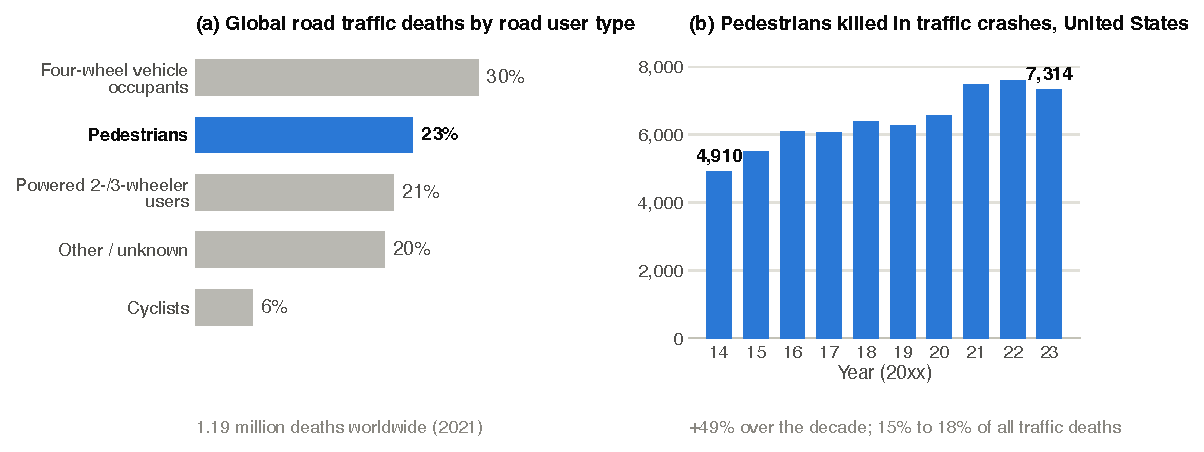
\includegraphics[width=\textwidth]{figures/fig1_pedestrian_statistics.pdf}
\caption{Pedestrians carry a disproportionate and growing share of road traffic casualties. (\textbf{a}) Global distribution of road traffic deaths by road user type; pedestrians account for 23\% of the 1.19 million deaths estimated for 2021, second only to occupants of four-wheeled vehicles~\citep{who2023roadsafety}. (\textbf{b}) Pedestrians killed in traffic crashes in the United States, 2014--2023; the annual count rose by roughly 49\% over the decade and the pedestrian share of all traffic fatalities grew from 15\% to 18\%, even though total traffic fatalities did not grow at the same rate~\citep{nhtsa2025pedestrians}. \label{fig:stats}}
\end{figure}

For the design of driver-assistance systems, the way this risk distributes matters as much as its size. In 2023, 84\% of pedestrian fatalities in the United States occurred in urban areas, 74\% at locations away from intersections, and 77\% in the dark~\citep{nhtsa2025pedestrians}. The typical fatal encounter is therefore not a signaled crosswalk at midday but an unsignaled crossing in city traffic, in poor light, where a driver has little time to react. Advanced driver-assistance systems (ADAS) and automated vehicles must anticipate such a crossing \emph{before} it begins rather than react once the pedestrian has stepped into the road, since braking distance at urban speeds consumes most of the interval between recognition and impact.

This is the task of pedestrian crossing-intention prediction: from a short observation of a pedestrian and of the ego-vehicle, estimate the probability that the pedestrian is about to cross~\citep{rasouli2019pie,kotseruba2021benchmark}. Intention prediction is not trajectory forecasting. A trajectory model extrapolates motion that has already begun, whereas an intention model must commit to a binary, safety-critical decision while the pedestrian is still on the curb, under substantial class imbalance, and fast enough for the decision to be actionable. The Pedestrian Intention Estimation (PIE) dataset~\citep{rasouli2019pie} has become the standard benchmark for this task, pairing on-board video with per-frame pedestrian bounding boxes, per-pedestrian crossing labels, and synchronized on-board-diagnostics (OBD) ego-vehicle speed, and most subsequent models are trained and compared on its fixed split by recording set.

Despite the maturity of this benchmark, three methodological weaknesses recur across the literature and motivate this paper. First, \textbf{temporal leakage is rarely checked}. Many PIE protocols anchor the observation window at the last annotated frame minus a fixed time-to-event offset, with no guarantee that the window ends before the pedestrian begins to cross. When the window overlaps frames in which the pedestrian is already crossing, the task quietly collapses from predicting an intention to detecting an event already in progress, and reported scores are inflated. The dataset authors' own recent benchmark notes a related misalignment between how intention and action samples are anchored~\citep{rasouli2024diving}, but a direct, quantified audit of window leakage on PIE is, to our knowledge, absent. Second, \textbf{recent state-of-the-art models are heavy}. Systems built on three to seven input streams require pose estimators, optical-flow networks, semantic segmentation, or depth models at inference time; these raise computational cost, add failure points, and are awkward to deploy on embedded automotive hardware~\citep{azarmi2025pipnet,xie2025gtranspdm}. Third, \textbf{evaluation is often thin}. Single fixed splits, single-seed ablations reported as conclusions, point estimates without confidence intervals, ground-truth bounding boxes substituted for a real detector, and unjustified hyperparameters are all common~\citep{rasouli2024diving,azarmi2024featureimportance}.

We deliberately do not claim that minimal-modality prediction is itself new. Prior work has already shown that a bounding box together with ego-vehicle motion can rival multimodal models on PIE, most directly PedCMT~\citep{chen2024pedcmt}, the pose-free ablation of GTransPDM~\citep{xie2025gtranspdm}, and the bounding-box-centric analysis of~\citet{achaji2022attention}. What has been missing is a demonstration that this result survives a leakage-free protocol and full statistical scrutiny, together with an explanation of \emph{why} so few inputs suffice. That is the gap we close.

Our contributions are:
\begin{itemize}
\item A quantified \textbf{temporal-leakage audit} of the common PIE protocol and a \textbf{leakage-free re-extraction} anchored at PIE's own crossing point, verified at 0\% window leakage (Sections~\ref{sec:leakage} and~\ref{sec:leakage-results}).
\item A \textbf{rigorous re-evaluation} of a parsimonious two-stream (bounding box + ego-speed) model: bootstrap and pedestrian-cluster confidence intervals, leave-one-set-out cross-validation, multi-seed ablations, a documented hyperparameter search, and a detector-in-the-loop test (Section~\ref{sec:results}).
\item A \textbf{four-family architecture study}. A bidirectional LSTM, a searched Transformer, a GRU, and an un-gated vanilla RNN, trained under one identical engine with matched search budgets, prove statistically indistinguishable on the primary metric, so \textbf{the input signal, not the architecture or its gating, decides} (Section~\ref{sec:architecture}).
\item A demonstration that the resulting predictor is \textbf{real-time}, at well under a millisecond per window, and that a full perception-to-prediction pipeline is bound by detection rather than by prediction (Sections~\ref{sec:latency} and~\ref{sec:detector}).
\end{itemize}

Throughout, we adopt the metric hierarchy \textbf{F1 $\rightarrow$ accuracy $\rightarrow$ AUC}: F1 is the imbalance-appropriate operating-point metric we report first, accuracy second, and ROC/PR-AUC as threshold-free corroboration.

The remainder of this paper is organized as follows. Section~\ref{sec:relatedwork} situates the work against PIE crossing-prediction baselines, recent multimodal approaches, and the pedestrian--vehicle interaction literature. Section~\ref{sec:methods} describes the PIE dataset, the leakage-free extraction protocol, the feature set, the four model families, and the shared training and evaluation procedure. Section~\ref{sec:results} reports the leakage audit, the main results with confidence intervals, the architecture comparison, the ablations, and the latency and detector-in-the-loop experiments. Section~\ref{sec:discussion} interprets these findings and states the limitations, and Section~\ref{sec:conclusions} concludes.

%=================================================================
\section{Related Work}
\label{sec:relatedwork}

\subsection{Datasets and Benchmarks for Pedestrian Crossing Behavior}

Research on pedestrian crossing prediction has been shaped by a small set of datasets recorded from a moving vehicle. The JAAD dataset introduced short clips annotated with pedestrian actions and contextual attributes around the moment of crossing~\citep{rasouli2017jaad}, and PIE extended this to roughly six hours of continuous urban driving with bounding-box tracks, behavioral tags, and synchronized on-board ego-vehicle OBD signals~\citep{rasouli2019pie}. Later datasets widened the scope: TITAN organized pedestrian and vehicle actions into a hierarchy of atomic and contextual labels~\citep{malla2020titan}, and the PSI benchmark added per-frame intent estimates together with free-text explanations of the reasoning collected from human drivers~\citep{chen2021psi}. These resources are multimodal by construction: they pair egocentric video with vehicle telemetry and human behavioral annotation, which is what makes crossing prediction a natural setting for studying interaction between road users.

Comparing methods fairly on these datasets depends on a shared protocol. The benchmark of Kotseruba et al.\ fixed how observation windows, prediction horizons, and train/test partitions are defined on PIE and JAAD, and released the PCPA model and reference scores against which later work is measured~\citep{kotseruba2021benchmark}. Even with a common benchmark, results do not transfer cleanly across datasets: a controlled study found that predictors trained on one dataset lose substantial accuracy when evaluated on another, pointing to dataset-specific bias rather than a solved task~\citep{gesnouin2022assessing}. Two surveys map the area in more detail and catalogue the proliferation of modalities and architectures~\citep{sharma2022survey,rasouli2024diving}.

\subsection{Models for Crossing-Intention Prediction}

Early crossing predictors borrowed sequence models from trajectory forecasting, where the LSTM~\citep{hochreiter1997lstm} and its bidirectional form~\citep{graves2005framewise} had already proved effective for pedestrian motion in crowded scenes~\citep{alahi2016social}. On PIE and JAAD the field then developed along three broad lines. Graph-based models represent the pedestrian, the scene, and their relations as nodes and edges: Pedestrian Graph+ pairs a graph convolutional encoder with a light backbone for fast inference~\citep{cadena2022pedgraph}, and related work models groups of pedestrians jointly to capture social context~\citep{zou2025group}. Attention- and transformer-based models then augmented or replaced recurrence: CAPformer applied self-attention to crossing-action prediction~\citep{lorenzo2021capformer}, PedFormer combined cross-modal attention with gated multitask learning~\citep{rasouli2023pedformer}, and GTransPDM embedded a positional-decoupling transformer over pose and graph features~\citep{xie2025gtranspdm}. The third line fuses progressively more input modalities: PCPA combines visual, motion, and ego cues through attention~\citep{kotseruba2021benchmark}; hybrid architectures stack appearance, pose, and trajectory streams~\citep{rasouli2022multimodal,piccoli2020fussinet}; and PIP-Net extends this to seven concurrent input streams including a categorical depth map and optical flow~\citep{azarmi2025pipnet}. Beyond these, recent work has explored uncertainty-aware and diffusion-based formulations~\citep{chen2024pedcmt,liu2025occlusion}, contextual feature fusion~\citep{azarmi2023local}, explicit coupling of intent and action~\citep{yao2021coupling,zhou2023learning}, explainable neuro-symbolic reasoning~\citep{melocastillo2025neurosymbolic}, and the most recent multi-context and sequential-plus-visual transformers~\citep{li2025mft,landry2025trajfusionnet,liang2024tcl}. Sensing beyond the on-board camera has also been tried, including wearable signals from a pedestrian's smartwatch~\citep{abbasi2023watchped} and infrastructure-side prediction at intersections~\citep{abdelrahman2025vrucipi}.

\subsection{Toward Minimal-Modality and Real-Time Prediction}

The prevailing trend adds modalities to chase accuracy, but a counter-current asks whether all of them earn their cost. The transformer backbone behind most recent models is itself expensive to run~\citep{vaswani2017attention}, and a crossing predictor must ultimately fit inside a tight frame budget on embedded automotive hardware; lighter recurrent units such as the GRU~\citep{cho2014gru} and compact graph backbones~\citep{cadena2022pedgraph} were partly motivated by that pressure. Several works establish that a minimal input is surprisingly strong. \citet{achaji2022attention} ask directly whether attention over bounding boxes is all that is needed, and report 91\% accuracy and 0.83 F1 on PIE from box geometry alone. As we show in Section~\ref{sec:leakage}, those numbers were measured under the pre-leakage observation-window protocol and overstate leakage-free performance. Closest to our own design, PedCMT predicts crossing from \emph{only} the pedestrian bounding box and ego-vehicle speed within a cross-modal transformer with uncertainty-aware multitask learning, and reports results on a par with, or superior to, models that rely on more inputs~\citep{chen2024pedcmt}; its released code confirms that no pose, flow, or scene encoder is used. The pose-free ablation of GTransPDM reaches comparable accuracy from bounding box and ego-motion alone~\citep{xie2025gtranspdm}, and the occlusion-aware diffusion model of~\citet{liu2025occlusion} likewise uses only bounding box and ego-velocity, though under an occlusion-specific, roughly one-frame-ahead protocol that is not directly comparable. Our work belongs to this minimal-modality line. Rather than claim minimal inputs as novel, we take them as an established design choice and ask how far two cheap streams, bounding-box motion and ego-speed, can go on the \emph{standard} PIE protocol once the evaluation is made leakage-free and statistically strict, and \emph{why} they suffice.

\subsection{Detection and Tracking in the Prediction Pipeline}

Most crossing-prediction studies evaluate on ground-truth bounding boxes, which skips the perception stage that any deployed system must include. In practice a predictor receives boxes from an object detector and identities from a multi-object tracker. Detection has moved from region-proposal networks~\citep{ren2015faster} to single-stage real-time detectors in the YOLO family~\citep{redmon2016yolo,jocher2025yolo}, and tracking-by-detection methods link boxes across frames, from the original SORT~\citep{bewley2016sort} and its appearance-aware extension DeepSORT~\citep{wojke2017deepsort} to ByteTrack, which recovers low-confidence detections to reduce identity switches~\citep{zhang2022bytetrack}. We pair a modern YOLO detector with ByteTrack to measure how a real perception front end, rather than ground-truth boxes, affects crossing prediction (Section~\ref{sec:detector}).

\subsection{Pedestrian--Vehicle Interaction and Implicit Communication}

Crossing is an interaction between the pedestrian and the approaching vehicle, not a solitary act. A substantial body of work in the multimodal-interaction community studies how automated vehicles can signal intent through external human--machine interfaces (eHMI), and how those signals change crossing decisions~\citep{riener2019guest,rouchitsas2019ehmi,alhawiti2024ehmi,rezwana2024interactions}. That literature mostly concerns \emph{explicit} communication from the vehicle to the pedestrian. Our result points the other way and complements it: the ego-vehicle's speed profile carries much of the predictive signal for whether a pedestrian will cross (Section~\ref{sec:main-result}), which suggests that the vehicle's own motion is an \emph{implicit} communication channel a model can read, while also cautioning that a model leaning on ego-speed partly reads the ego-driver's anticipation rather than the pedestrian alone (Section~\ref{sec:limitations}).

\subsection{Research Gaps Addressed in This Work}

Four gaps recur across this literature. First, the standard windowing protocol is rarely audited for \textbf{temporal leakage}: the dataset authors' own benchmark notes that intention labels anchored at a crossing point and action samples anchored by a fixed time-to-event do not always overlap, so reported scores can reflect the detection of crossings already in progress rather than their prediction~\citep{rasouli2024diving}. Second, accuracy gains are usually bought with \textbf{heavier modality stacks} (pose, flow, segmentation, or depth) whose real-time cost on embedded hardware is seldom measured~\citep{azarmi2025pipnet,cadena2022pedgraph}. Third, results are often reported as a \textbf{single point estimate} from one split and one seed, with no confidence interval or cross-set validation, and typically assume \textbf{ground-truth boxes}, leaving the effect of real detection and tracking noise unquantified. Fourth, the modalities that matter are seldom isolated: a recent context-aware feature-importance analysis finds that bounding box and ego-speed dominate the prediction and cautions that reliance on ego-speed can induce a driver-side bias in yielding scenarios~\citep{azarmi2024featureimportance}. The remainder of this paper addresses these gaps on the standard PIE protocol: we audit and remove the leakage, hold the model to two cheap streams, and attach an interval to every comparison we draw.


%=================================================================
\section{Materials and Methods}
\label{sec:methods}

\subsection{Overview}

The study has a deliberately narrow design. One dataset, one windowing protocol, one input representation, and one training engine are held fixed; the only things that vary are the factors under test: the anchoring rule that defines an observation window, the presence of the ego-speed stream, the temporal encoder, the observation length, and the prediction horizon. Figure~\ref{fig:system}a shows the resulting model. Everything outside the dashed block is frozen across every experiment reported here, which is what allows a difference between two rows of a results table to be attributed to a single design choice rather than to an accumulation of incidental differences.

\begin{figure}[H]
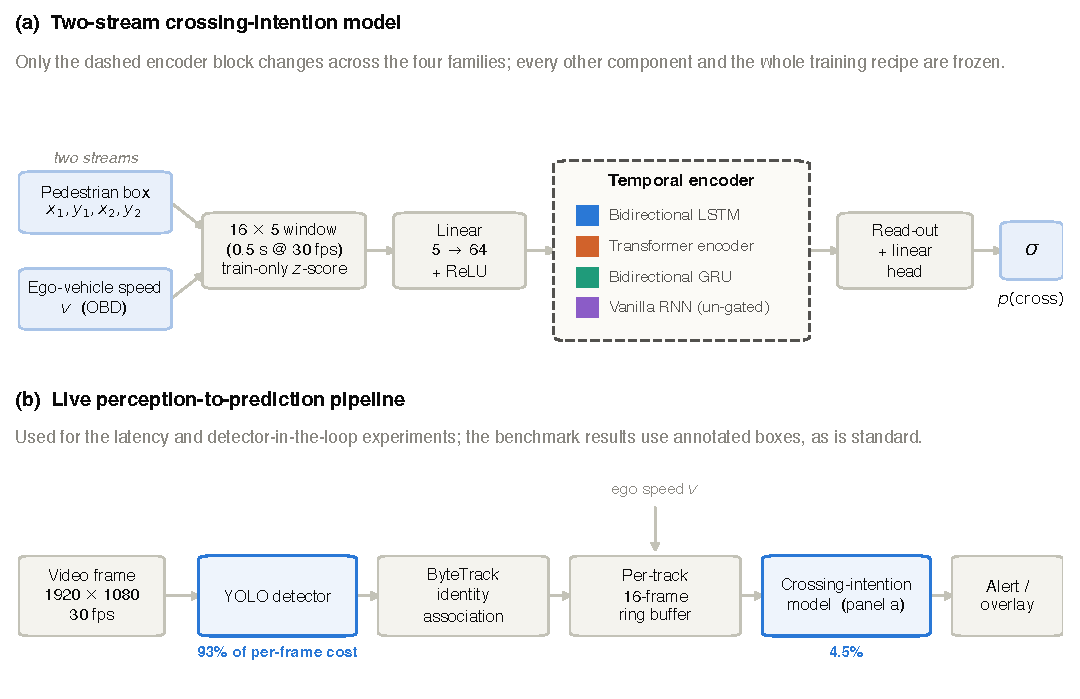
\includegraphics[width=\textwidth]{figures/fig2_system.pdf}
\caption{The model and the pipeline it runs inside. (\textbf{a}) The two-stream crossing-intention model. A 16-frame window of bounding-box corners and ego-vehicle speed is standardized, projected, encoded by one of four temporal architectures, and read out through a linear head. Only the dashed block changes across the four families. (\textbf{b}) The live perception-to-prediction pipeline used for the latency and detector-in-the-loop experiments, annotated with each stage's measured share of per-frame cost. The benchmark results in Section~\ref{sec:results} use annotated boxes, as is standard on PIE.\label{fig:system}}
\end{figure}

\subsection{The PIE Dataset and Splits}
\label{sec:dataset}

PIE~\citep{rasouli2019pie} comprises roughly six hours of on-board video (1920$\times$1080 at 30\,fps) recorded in Toronto traffic across six recording sets (set01--set06). Each annotated pedestrian carries a per-frame bounding-box track, a set of behavioral attributes including a per-frame \texttt{cross} state, a per-pedestrian binary crossing label and, critically for this work, a \texttt{crossing\_point} event frame marking when the crossing begins. Ego-vehicle speed is recorded synchronously from the vehicle's on-board diagnostics (OBD) port, giving a second modality that is available at inference time without any additional perception.

We use the standard benchmark split by recording set: train on set01, set02, and set04; validate on set05 and set06; test on set03. Splitting by recording set rather than at random is what prevents identity- and scene-level leakage, since a pedestrian, a video, and a stretch of road each belong to exactly one split. This is the partition used by the reference benchmark~\citep{kotseruba2021benchmark} and by the baselines we compare against, so our numbers are protocol-comparable to theirs.

\subsection{Temporal Leakage and the Leakage-Free Protocol}
\label{sec:leakage}

\subsubsection{The Problem with Anchoring at the End of a Track}

The prevailing extraction procedure places each observation window at the last annotated frame of a pedestrian's track, minus a fixed time-to-event (TTE) offset. The difficulty is that the end of an annotated track has no defined relationship to the moment the pedestrian steps into the road. A track may continue for many seconds after the crossing begins, in which case a window offset backwards from its end still lands well inside the crossing (Figure~\ref{fig:protocol}a). When that happens, the model is shown frames in which the pedestrian is visibly already crossing, and the task silently changes from predicting an intention to recognizing an event in progress. Any score measured that way is an optimistic estimate of what the model would achieve in deployment, where no such frames exist yet.

This is not a hypothetical concern: PIE's per-frame \texttt{cross} attribute lets it be measured directly. The original parsing script in our own earlier pipeline retained only the \texttt{action} attribute and discarded \texttt{cross}, which is precisely why the problem went unnoticed for as long as it did. We re-parsed the annotation XML to recover the per-frame \texttt{cross} state (\emph{not-crossing} / \emph{crossing} / \emph{crossing-irrelevant}) and used it as the ground truth for the audit reported in Section~\ref{sec:leakage-results}.

\subsubsection{Re-Anchoring at the Crossing Point}

The fix follows from the diagnosis. Instead of measuring backwards from the end of a track, we measure backwards from the event itself. For each pedestrian we take the contiguous track segment containing \texttt{crossing\_point}, truncate it at that frame inclusive, and slide 16-frame windows across the remaining history at 50\% overlap, keeping only those whose last observed frame falls a TTE of $[30, 60]$ frames (1--2\,s) \emph{before} the crossing point (Figure~\ref{fig:protocol}b). Non-crossing pedestrians contribute windows from their full track under the same window length and stride. Pedestrians whose usable track is shorter than the window plus the minimum look-ahead (107 of 1,374, or 7.8\%) are excluded, since no leakage-free window can be formed for them.

Two properties make this leakage-free by construction rather than by inspection. First, \texttt{crossing\_point} coincides with the first frame labeled \texttt{cross}~=~\emph{crossing} for 516 of 519 crossing pedestrians (99.4\%) and never precedes it, so it is a faithful marker of onset. Second, requiring at least 30 frames of look-ahead means the last observed frame is at least a full second before that marker. Table~\ref{tab:dataset} summarizes what changes. The leakage-free protocol is also the larger dataset: sliding windows across pre-crossing history rather than taking one window per track increases the sample 3.5-fold, from 1,389 to 4,906 windows.

\begin{table}[H]
\caption{Track-end versus crossing-point anchoring on PIE. Re-anchoring at the crossing-point event removes all window leakage and, because it slides windows across each pedestrian's pre-crossing history rather than taking a single window per track, also grows the sample 3.5-fold. $\mathrm{pos\_weight}$ is the positive-class weight used in the training loss; for the crossing-point protocol it is the training split's negative-to-positive ratio, 1366/812.\label{tab:dataset}}
\begin{tabularx}{\textwidth}{lCCCC}
\toprule
\textbf{Protocol} & \textbf{Windows (train/val/test)} & \textbf{Positive Rate} & \textbf{Window Leakage} & \textbf{$\mathrm{pos\_weight}$}\\
\midrule
Track-end anchor & 1{,}389 (616/186/587) & 41.0\% & 387 of 570 (67.9\%) & 1.44\\
\textbf{Crossing-point anchor} & \textbf{4{,}906 (2{,}178/634/2{,}094)} & 33.6\% & \textbf{0 of 4{,}906 (0.0\%)} & 1.682\\
\bottomrule
\end{tabularx}
\end{table}

\begin{figure}[H]
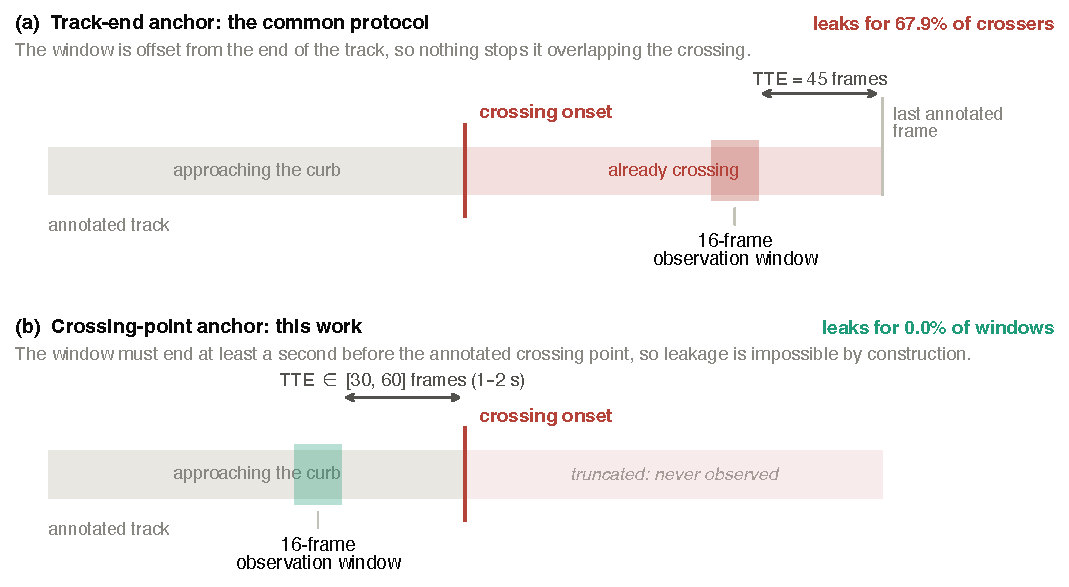
\includegraphics[width=\textwidth]{figures/fig3_protocol.pdf}
\caption{Where the observation window lands under each anchoring rule, for one crossing pedestrian. (\textbf{a}) Anchoring at the last annotated frame minus a fixed time-to-event offset places no constraint on the crossing onset; on PIE the window then overlaps the crossing for 67.9\% of crossing pedestrians, and the model observes an event it is nominally predicting. (\textbf{b}) Anchoring at PIE's own \texttt{crossing\_point} and requiring a look-ahead of 30--60 frames makes leakage impossible: every window ends at least a second before the pedestrian steps into the road. Frame positions are illustrative; the offsets and leakage rates are measured.\label{fig:protocol}}
\end{figure}

\subsection{Features and Preprocessing}
\label{sec:features}

Every model receives the same input: a 16-frame window (0.5\,s at 30\,fps) of a five-dimensional vector $[x_1, y_1, x_2, y_2, v]$, where $(x_1, y_1, x_2, y_2)$ are the pedestrian's bounding-box corners and $v$ is the ego-vehicle speed. Box coordinates are kept in raw PIE pixel units on the 1920$\times$1080 image plane and are deliberately \emph{not} normalized by image size; the network sees absolute geometry, and the standardization step below handles scaling.

Each of the five features is standardized by its own $z$-score, $(x - \mu)/\sigma$, with $\mu$ and $\sigma$ computed on the training split alone and then applied unchanged to validation and test. Computing these statistics over the whole dataset would leak distributional information about the evaluation sets into training; keeping them train-only is a small discipline that costs nothing and removes a real confound. The bounding-box-only ablation of Section~\ref{sec:ego-ablation} drops $v$ and is otherwise identical, giving a four-dimensional input.

Unless stated otherwise, the decision threshold is 0.5 applied to the sigmoid output, which is what makes our numbers directly comparable with the published baselines in Table~\ref{tab:baselines}.

\subsection{Model Architectures}
\label{sec:architectures}

All four families share one minimal wrapper: a linear projection of the five input features to 64 dimensions with a ReLU nonlinearity, a temporal encoder, a read-out of the final (or pooled) time step, and a linear classification head producing a single logit. Only the encoder differs. Every network is trained from scratch; none uses pretrained weights, which keeps the comparison free of differences in pretraining data or scale.

\begin{itemize}
\item \textbf{BiLSTM}: a two-layer bidirectional long short-term memory network~\citep{hochreiter1997lstm,schuster1997bilstm} with last-step read-out. This is the reference model, and the one we report as the headline system.
\item \textbf{Transformer}: a small pre-layer-norm Transformer encoder~\citep{vaswani2017attention,xiong2020prelayernorm}, whose width, depth, head count, pooling strategy, and positional encoding were searched (Section~\ref{sec:training}).
\item \textbf{GRU}: the BiLSTM with its cell replaced by a gated recurrent unit~\citep{cho2014gru,chung2014gru} and nothing else changed. This isolates the choice of \emph{which} gated cell is used.
\item \textbf{Vanilla RNN}: the BiLSTM with gating removed entirely: a bidirectional tanh (Elman) recurrent network~\citep{elman1990rnn,rumelhart1986backprop}. This isolates \emph{gating itself}.
\end{itemize}

The three recurrent families form a deliberate ladder. Moving from the LSTM to the GRU changes the gating mechanism; moving from the GRU to the vanilla RNN removes gating altogether. If recurrent machinery is what makes this task work, performance should fall at each rung. Two further BiLSTM variants serve as ablations: a bounding-box-only model that drops the ego-speed stream, and a model with additive temporal attention over the recurrent states~\citep{bahdanau2015attention}. Table~\ref{tab:hparams} lists the settings selected for each headline model.

\begin{table}[H]
\caption{Searched settings for each headline model. Everything not listed is frozen and identical across all families: batch size 32, at most 100 epochs, early stopping with patience 15, train-only $z$-score standardization, Adam, weight decay $10^{-5}$, and a class weight anchored at 1.682. ``Width'' is the recurrent hidden size (the read-out is twice this, being bidirectional) or the Transformer's model and feed-forward dimensions. $\tau$ is the operating threshold, tuned on validation data only.\label{tab:hparams}}
\begin{tabularx}{\textwidth}{Xlccccc}
\toprule
\textbf{Model} & \textbf{Cell} & \textbf{Width} & \textbf{Layers} & \textbf{Drop.} & \textbf{LR} & \textbf{$\tau$}\\
\midrule
BiLSTM (baseline) & LSTM & 128 & 2 & 0.3 & $10^{-3}$ & 0.50\\
BiLSTM-F1 & LSTM & 256 & 2 & 0.3 & $10^{-3}$ & 0.52\\
Transformer (searched) & attention (4 heads) & 128/512 & 4 & 0.1 & $10^{-3}$ & 0.50\\
Transformer-F1 & attention (4 heads) & 128/512 & 4 & 0.1 & $10^{-3}$ & 0.65\\
GRU-F1 & GRU & 256 & 2 & 0.3 & $5{\cdot}10^{-4}$ & 0.53\\
Vanilla RNN-F1 & Elman (tanh) & 256 & 2 & 0.2 & $10^{-4}$ & 0.53\\
\bottomrule
\end{tabularx}
\end{table}

\subsection{Training Protocol and Hyperparameter Search}
\label{sec:training}

Every family is trained through a single model-agnostic engine, so that the recipe cannot drift between architectures. The loss is binary cross-entropy with a positive-class weight of 1.682, the training split's negative-to-positive ratio, applied only in the training gradient and never in evaluation. Optimization uses Adam~\citep{kingma2015adam} with weight decay $10^{-5}$ (AdamW~\citep{loshchilov2019adamw} in some Transformer search stages), batch size 32, at most 100 epochs, early stopping with patience 15, and a plateau learning-rate schedule. Every configuration is trained with five seeds (42, 0, 1, 2, 3). The test set is evaluated exactly once per model, on the checkpoint selected by validation performance, by a single designated script.

Hyperparameters are searched rather than asserted, and the search is reported whether or not it changed anything. The BiLSTM received a 36-configuration grid over learning rate, dropout, hidden size, and depth, selected on validation AUC alone. The Transformer, having more architectural freedom, received a larger 78-configuration staged search over both architecture and recipe, with its winner chosen by five-seed mean validation performance. The GRU and the vanilla RNN each received the \emph{identical} search budget as the BiLSTM. This symmetry matters more than the searches individually: a comparison in which one family is tuned and another is not measures tuning effort, not architecture.

\subsection{Metric Hierarchy and F1-First Selection}
\label{sec:metrics}

We report F1 first, accuracy second, and ROC-AUC and PR-AUC as threshold-free corroboration. The ordering is a considered choice for an imbalanced, safety-critical binary decision. A deployed system must commit to a threshold, so a metric that summarizes performance at an operating point is more informative than one that averages over all of them; and with roughly one window in three positive, accuracy alone rewards a model that leans toward the majority class. AUC remains valuable precisely because it is threshold-free, which makes it a good check on whether an F1 result is an artifact of threshold placement.

Making F1 the primary metric has three consequences for model selection, applied symmetrically to all four families: the operating threshold $\tau$ is tuned on validation data only (it landed near 0.5 for most models, so the reported figures remain broadly threshold-0.5-comparable); each family's configuration is re-selected by validation F1; and checkpoints are taken at best validation F1 rather than best validation AUC. Where a model selected under the older AUC-first rule is also reported, it is labeled as such, since the two rules can select different configurations from the same search.

\subsection{Evaluation and Statistical Procedure}
\label{sec:evaluation}

Point estimates are per-seed means over the five seeds; we report the standard deviation across seeds where it aids interpretation. Because a single number invites over-reading, every claim of a difference is backed by an interval.

Uncertainty on the 2,094 test windows is quantified with a 10,000-resample bootstrap. Windows drawn from the same pedestrian are not independent. They overlap in time and share an identity, a scene, and a behavior, so a bootstrap that resamples windows will understate uncertainty. We therefore also report a \emph{pedestrian-cluster} bootstrap that resamples the 541 test pedestrians as whole units, and we treat that stricter interval as the primary evidence. Comparisons between two models are made as \emph{paired} bootstraps on the identical resamples, which removes the shared difficulty of the test set from the contrast.

Generalization beyond the fixed split is assessed by leave-one-set-out (LOSO) cross-validation, rotating the held-out recording set across all six. Where a deployable five-seed probability ensemble is reported, it is labeled as such and never mixed into a per-seed comparison table, since the two are different statistics and the ensemble is systematically the more favorable one.

\subsection{Live Perception-to-Prediction Pipeline}
\label{sec:pipeline}

For the deployment analysis we built the pipeline of Figure~\ref{fig:system}b. Pedestrians are detected with a YOLO-family single-stage detector~\citep{redmon2016yolo,jocher2025yolo}, associated across frames by ByteTrack~\citep{zhang2022bytetrack}, and buffered per track into the same 16-frame window of $[x_1, y_1, x_2, y_2, v]$ the offline models consume, with $v$ read from the vehicle rather than from vision. This pipeline is used for the latency measurement of Section~\ref{sec:latency}, the detector-in-the-loop experiment of Section~\ref{sec:detector}, and the qualitative examples of Section~\ref{sec:qualitative}; the benchmark results use annotated boxes, as every comparable study does.

\subsection{Implementation and Reproducibility}
\label{sec:implementation}

All models are implemented in PyTorch~\citep{paszke2019pytorch}. Timing measurements were taken on an Apple M4 CPU with 50 warm-up and 1,000 timed forward passes per configuration. One reproducibility caveat is worth recording because it cost us time to find: training \texttt{nn.LSTM} on Apple's Metal Performance Shaders backend proved dependent on process history, so the same configuration and seed can produce different results depending on what ran earlier in the same process. Recurrent runs that must reproduce exactly were therefore executed on CPU, where training is bit-reproducible; Transformer training did not show this behavior.

%=================================================================
\section{Results}
\label{sec:results}

\subsection{The Temporal-Leakage Audit}
\label{sec:leakage-results}

Auditing the track-end protocol against the recovered per-frame \texttt{cross} state produces the paper's first and most consequential finding. Of 570 crossing pedestrians, 387 (67.9\%) have at least one frame inside the observation window in which they are already crossing, and 369 (64.7\%) are already crossing in \emph{all sixteen} frames. Only 183 crossers (32.1\%) have a genuinely clean window (Figure~\ref{fig:leakage}a). For roughly two-thirds of the positive class, then, what is reported as prediction is the detection of an event already under way.

A second, subtler shortcut accompanies the first. The single bounding box at the last observed frame separates crossers from non-crossers on its own, with no temporal information at all: rank-biserial correlations of $+0.65$ for box area, $+0.63$ for box height, and $+0.49$ for the box's bottom edge (Figure~\ref{fig:leakage}b). This is what one would expect if the model is looking at pedestrians who are already in the road: they are nearer the camera, hence larger and lower in the frame.

Re-running the identical audit on the crossing-point protocol confirms 0 of 4,906 windows leaking, and the static shortcut weakens sharply, with every effect size falling below 0.3 (box area $0.25$, height $0.21$, bottom edge $0.09$). The signal that remains must live in the temporal dynamics rather than in a static giveaway. Two details of the leaky protocol are worth recording as diagnostics for other datasets: the median gap between the window's end and the crossing onset was $+182$ frames, six seconds \emph{into} the crossing, and models trained on it converged suspiciously early, typically by epoch~3.

\begin{figure}[H]
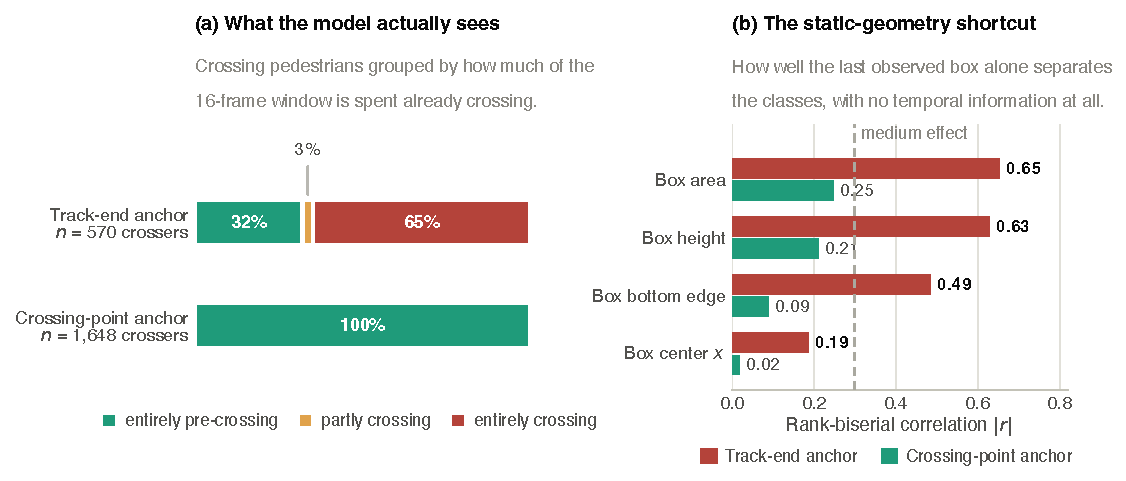
\includegraphics[width=\textwidth]{figures/fig4_leakage.pdf}
\caption{The temporal-leakage audit, computed from PIE's own per-frame \texttt{cross} annotations. (\textbf{a}) Crossing pedestrians grouped by how much of the 16-frame observation window is already spent crossing. Under the track-end anchor, 65\% of crossers are already crossing in every observed frame and only 32\% have a clean window; under the crossing-point anchor, every window is clean by construction. (\textbf{b}) How well the single bounding box at the last observed frame separates crossers from non-crossers, with no temporal information at all. Under the track-end anchor, box area and height are large effects; re-anchoring removes the shortcut, leaving all effects below the conventional medium threshold.\label{fig:leakage}}
\end{figure}

\subsection{Main Result}
\label{sec:main-result}

On the leakage-free protocol, the two-stream BiLSTM reaches test F1 0.844, accuracy 0.897, and ROC-AUC 0.940 under F1-first optimization (Table~\ref{tab:families}). Its 10,000-resample bootstrap gives a 95\% AUC interval of $[0.92, 0.95]$ at the window level and $[0.92, 0.96]$ over pedestrian clusters, with PR-AUC 0.876.

Removing the leakage barely moved this model's AUC, from 0.931 on the leaky protocol to 0.913 for the same seed and 0.932~$\pm$~0.011 over five seeds, while moving convergence from epoch~3 to a believable epoch~17. That is worth stating plainly, because it is the opposite of what one might assume: the correction is methodological rather than a deflation of the score. What changed is what the number \emph{means}. A model that scored 0.93 by recognizing crossings in progress and a model that scores 0.93 by anticipating them a second in advance are different systems that happen to share a digit.

We also checked that the new protocol is not simply an easier one. Per-pedestrian AUC (0.914) matches per-window AUC (0.913), so the result is not an artifact of some pedestrians contributing many correlated windows. The additional short tracks admitted by the 50\% overlap are \emph{harder} than the rest, not easier (AUC 0.863 for tracks of 46--75 frames, against 0.919 for longer ones), so the larger sample is not a diluted one. Figure~\ref{fig:curves} shows the full ROC and precision--recall curves for all four families.

\begin{figure}[H]
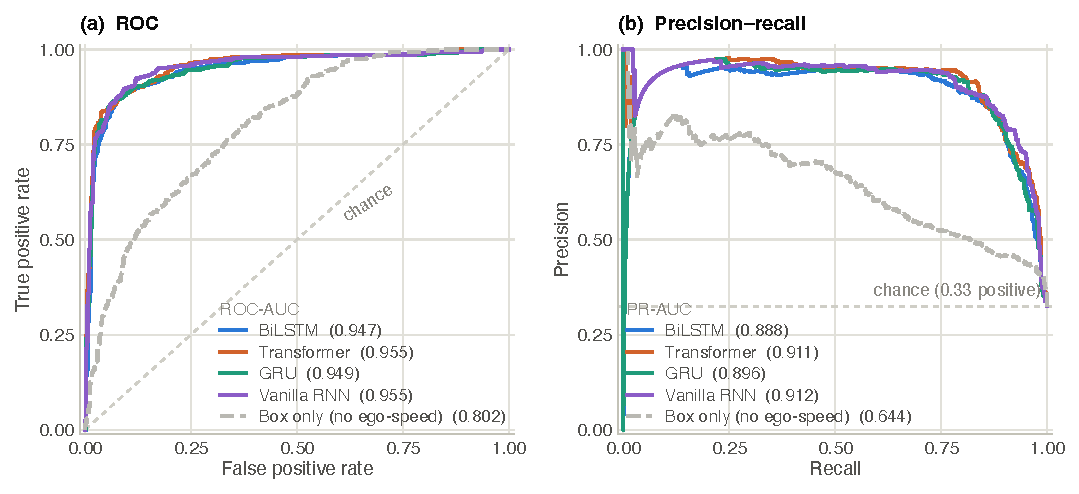
\includegraphics[width=\textwidth]{figures/fig5_curves.pdf}
\caption{(\textbf{a}) ROC and (\textbf{b}) precision--recall curves for the four F1-optimized family headliners on the 2,094 leakage-free test windows, with the bounding-box-only ablation as the context series. Curves are the five-seed probability ensemble; parenthesized values in each legend are the corresponding areas. The four families lie almost exactly on top of one another over the whole operating range, while removing the ego-speed stream pulls the curve down and away from them.\label{fig:curves}}
\end{figure}

\subsection{Does the Architecture Matter?}
\label{sec:architecture}

Table~\ref{tab:families} reports all four families trained under the identical engine, and Figure~\ref{fig:forest} gives the paired contrasts with pedestrian-cluster confidence intervals. Three results follow, and they are best read in order.

First, on ROC-AUC the searched Transformer is genuinely the best model in the table (0.950), and a paired bootstrap on the identical test windows confirms it beats the BiLSTM ($\Delta$AUC $= +0.0135$, 95\% CI $[+0.0097, +0.0174]$).

Second, that win belongs to the search rather than to attention. A Transformer trained with the BiLSTM's own un-searched recipe merely ties it ($\Delta$AUC $= +0.0005$, interval spanning zero). The same architecture family therefore either beats or ties the recurrent baseline depending only on whether it was tuned, which is a useful reminder that an architecture comparison with asymmetric search budgets measures the budgets.

Third, and this is the central claim: \textbf{on the primary metric the four families are statistically indistinguishable}. Every cross-family $\Delta$F1 interval spans zero (Figure~\ref{fig:forest}a): the GRU against the BiLSTM ($+0.0071$), the vanilla RNN against the BiLSTM ($+0.0033$), the Transformer against the BiLSTM ($+0.0008$), and each remaining pair likewise. Removing the LSTM's gating entirely costs nothing over a 0.5\,s window; the un-gated network even ties the searched Transformer on AUC ($\Delta$AUC $-0.0013$, interval spanning zero) while being the smallest and fastest family in the study.

An equivalence claim is only as good as the power of the test behind it, so we checked that the same procedure can detect differences when they exist. It can. Each F1-optimized model beats its own family's AUC-selected baseline by an interval that clears zero (Figure~\ref{fig:forest}a, lower group), and several AUC contrasts separate cleanly (Figure~\ref{fig:forest}b). The ties are ties, not a failure to measure.

\begin{table}[H]
\caption{All four architecture families on the leakage-free PIE test set (set03; 2,094 windows, 32.5\% positive). Values are per-seed means over five seeds; ($\star$) marks the headline model of each family. Metrics are ordered F1, then accuracy, then AUC. All models use two input streams (bounding box and ego-vehicle speed) except where noted.\label{tab:families}}
\begin{tabularx}{\textwidth}{lXcccc}
\toprule
\textbf{Family} & \textbf{Model} & \textbf{Params} & \textbf{F1} & \textbf{Acc} & \textbf{AUC}\\
\midrule
BiLSTM & BiLSTM (baseline, AUC-selected) & 594{,}561 & 0.828 & 0.883 & 0.932\\
BiLSTM & BiLSTM, bounding-box only (4-D) & 594{,}497 & 0.551 & 0.744 & 0.753\\
BiLSTM & BiLSTM + temporal attention & 611{,}265 & 0.821 & 0.879 & 0.925\\
BiLSTM & BiLSTM-F1 ($\star$) & 2{,}237{,}313 & \textbf{0.844} & 0.897 & 0.940\\
Transformer & Transformer, un-searched & 268{,}417 & 0.821 & 0.878 & 0.942\\
Transformer & Transformer, searched ($\star$) & 794{,}241 & 0.845 & 0.894 & \textbf{0.950}\\
Transformer & Transformer-F1 & 794{,}241 & 0.847 & 0.896 & 0.947\\
GRU & GRU-F1 ($\star$) & 1{,}678{,}209 & 0.849 & 0.901 & 0.941\\
RNN & Vanilla RNN-F1 ($\star$) & 560{,}001 & \textbf{0.852} & 0.902 & 0.948\\
\bottomrule
\end{tabularx}
\end{table}

\begin{figure}[H]
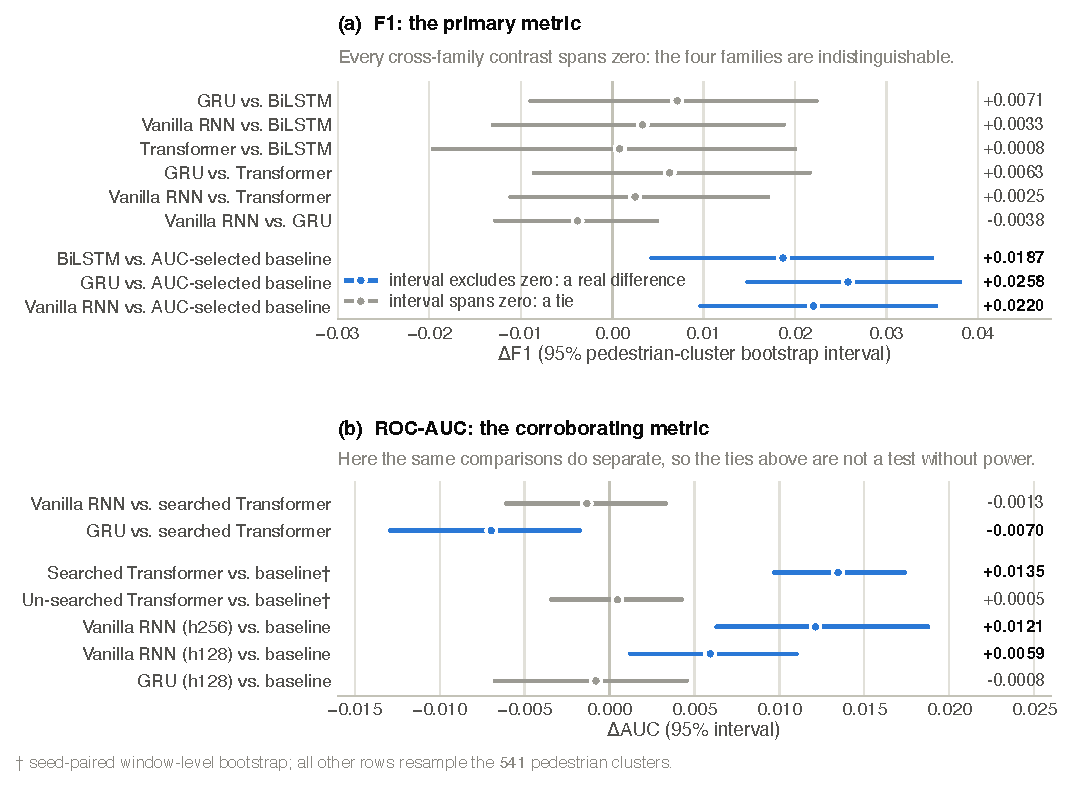
\includegraphics[width=\textwidth]{figures/fig6_forest.pdf}
\caption{Paired contrasts between models on the identical test windows, with 95\% intervals from a 10,000-resample bootstrap over the 541 test pedestrians. (\textbf{a}) On F1, the primary metric, every cross-family contrast spans zero: the four families are indistinguishable. The lower group shows the same procedure detecting a real effect: each F1-optimized model beats its own family's AUC-selected baseline, which establishes that the ties above are not simply a test without power. (\textbf{b}) On ROC-AUC the same models do separate in places, notably the searched Transformer against the baseline. Rows marked $\dagger$ use a seed-paired window-level bootstrap; all others resample pedestrian clusters.\label{fig:forest}}
\end{figure}

\subsection{Comparison with Published Baselines}
\label{sec:baselines}

Table~\ref{tab:baselines} places our models beside published PIE results on the standard protocol, with a column counting input streams. On F1, our primary metric, the two-stream models reach 0.844--0.852, ahead of most multimodal baselines and within about 0.02 of the ceiling set by PedFormer (0.87), using two inputs instead of three to seven. On AUC they lead the table at 0.94--0.95. On accuracy we sit honestly mid-band: 0.90 against PedFormer's 0.93.

We report that accuracy gap rather than omitting it, and it is worth being clear about why. A model that led every column of a benchmark table while using the fewest inputs would invite the suspicion that its evaluation was easier, and the leakage audit in Section~\ref{sec:leakage-results} is precisely a demonstration that such suspicions are sometimes correct. Leading on two metrics and trailing on a third is the profile of a real result.

Two recent systems are discussed but not tabulated. PIP-Net~\citep{azarmi2025pipnet} uses a custom data split rather than the standard one, so its figures are not protocol-comparable. The occlusion-aware diffusion model of~\citet{liu2025occlusion} evaluates under an occlusion-specific, roughly one-frame-ahead protocol; it is relevant as a precedent for minimal modality, not as a comparison row.

\begin{table}[H]
\caption{Crossing-prediction performance on PIE under the standard protocol (train set01/02/04, validate set05/06, test set03). Baseline figures are as reported by the cited sources. Our rows are per-seed means over five seeds at threshold 0.5.\label{tab:baselines}}
\begin{tabularx}{\textwidth}{lcccX}
\toprule
\textbf{Method} & \textbf{Acc} & \textbf{AUC} & \textbf{F1} & \textbf{Modalities (Streams)}\\
\midrule
PCPA~\citep{kotseruba2021benchmark} & 0.87 & 0.86 & 0.77 & box + pose + context + speed (4)\\
Pedestrian Graph+~\citep{cadena2022pedgraph} & 0.89 & 0.90 & 0.81 & pose graph + ego (2--3)\\
IntFormer~\citep{lorenzo2021intformer} & 0.89 & 0.92 & 0.81 & multimodal\\
PIT~\citep{zhou2023pit} & 0.91 & 0.92 & 0.82 & multimodal\\
BiPed~\citep{rasouli2023pedformer} & 0.91 & 0.90 & 0.85 & multimodal\\
PedFormer~\citep{rasouli2023pedformer} & \textbf{0.93} & 0.90 & \textbf{0.87} & multimodal (multitask)\\
GTransPDM~\citep{xie2025gtranspdm} & 0.90 & 0.87 & 0.82 & box + pose + ego (3)\\
GTransPDM without pose~\citep{xie2025gtranspdm} & 0.92 & 0.90 & 0.86 & box + ego (2)\\
PedCMT~\citep{chen2024pedcmt} & 0.92 & --- & --- & box + ego-speed (2)\\
MFT~\citep{li2025mft} & 0.90 & 0.94 & 0.83 & 4 context streams\\
\midrule
BiLSTM-F1 (ours) & 0.897 & 0.940 & 0.844 & \textbf{box + ego-speed (2)}\\
Transformer-F1 (ours) & 0.896 & 0.947 & 0.847 & \textbf{box + ego-speed (2)}\\
GRU-F1 (ours) & 0.901 & 0.941 & 0.849 & \textbf{box + ego-speed (2)}\\
Vanilla RNN-F1 (ours) & 0.902 & \textbf{0.948} & \textbf{0.852} & \textbf{box + ego-speed (2)}\\
\bottomrule
\end{tabularx}
\end{table}

\subsection{Which Input Carries the Signal?}
\label{sec:ego-ablation}

Dropping the ego-speed stream from an otherwise identical BiLSTM collapses it (Figure~\ref{fig:ablations}a): AUC falls from 0.932 to 0.753, F1 from 0.828 to 0.551, and accuracy from 0.883 to 0.744. A loss of 0.18 AUC from removing one of two inputs is not a marginal effect, and it identifies ego-vehicle speed as the dominant predictor, consistent with the independent context-aware feature-importance analysis of~\citet{azarmi2024featureimportance}. Adding temporal attention to the same model, by contrast, changes nothing on clean data (AUC 0.925 against 0.932).

Read alongside the four-family equivalence, this is the paper's mechanistic explanation. The predictive content lives in the ego-speed profile and in coarse bounding-box dynamics, both of which are legible within half a second. There is no long-range temporal structure for a more sophisticated encoder to exploit, which is why swapping the encoder changes so little and why removing the second input stream changes so much.

The collapse is also the other half of the leakage story. Once the static-geometry shortcut has been removed, a model given only bounding boxes has very little left to work with, which is a fair description of the task as it actually stands.

\subsection{Prediction Horizon and Observation Length}
\label{sec:horizon}

How far ahead the model must predict matters; how long it gets to observe does not.

AUC declines monotonically as the horizon lengthens, from 0.961 at 1.0\,s to 0.946 at 1.5\,s and 0.919 at 2.0\,s, with every pairwise paired $t$-test significant ($p \le 0.004$) and Kruskal--Wallis $p = 0.002$ (Figure~\ref{fig:ablations}b). Because a longer horizon requires a longer usable track and so changes which pedestrians are eligible, we repeated the comparison on a matched cohort: the same 493 test pedestrians at all three horizons, with only the observed window moving. The decline survives essentially unchanged (sample effect $\le 0.002$ AUC), so it reflects the task rather than the sampling. This is the behavior one wants from a genuine predictor, and it corrects an earlier ``insensitive to horizon'' conclusion of our own that was itself a leakage artifact: a model detecting crossings already in progress is indifferent to a nominal horizon it is not really respecting.

Observation length behaves in the opposite way. Over 8, 16, and 30 frames the baseline's AUC moves only from 0.931 to 0.933 to 0.937, a spread smaller than seed noise (all pairwise $p > 0.21$). Extending the window further, to 32 and 64 frames across all four F1-optimized families, makes matters slightly worse rather than better: F1 declines monotonically for every family (Figure~\ref{fig:ablations}c). Half a second already carries the available dynamics, and additional history mainly dilutes it. This justifies the 16-frame window as a design choice rather than an arbitrary one, and it is convenient for deployment, since a shorter window means a shorter wait before a newly detected pedestrian can be scored.

One asymmetry appears at the longest window and is worth flagging honestly. At 64 frames the un-gated vanilla RNN alone falls behind, losing 0.050 F1 against its own 16-frame result, roughly double the decline of the gated cells, and posting the lowest F1, accuracy, and AUC of the four. Per-seed intervals still overlap, so this is directional rather than a bootstrap-confirmed loss, but it points the way one would expect: gating is redundant over half a second and begins to earn its keep by about two seconds. The equivalence we report is horizon-bounded, and we say so.

\begin{figure}[H]
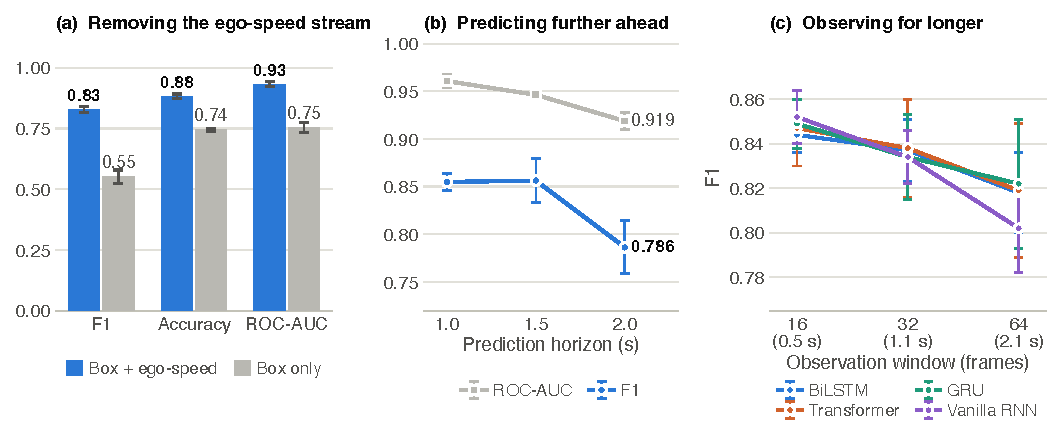
\includegraphics[width=\textwidth]{figures/fig7_ablations.pdf}
\caption{What the model needs, and how far ahead it can see. (\textbf{a}) Removing the ego-speed stream from an otherwise identical BiLSTM. (\textbf{b}) Performance against prediction horizon on a matched pedestrian cohort, holding the test population fixed at 493 pedestrians across all three horizons so that the decline cannot be a sampling artifact. (\textbf{c}) F1 against observation-window length for the four F1-optimized families; longer windows do not help any of them, and at 64 frames the un-gated vanilla RNN declines fastest. Markers are five-seed means; whiskers are $\pm$1 standard deviation across seeds.\label{fig:ablations}}
\end{figure}

\subsection{Cross-Set Generalization}
\label{sec:loso}

Rotating the held-out recording set across all six folds gives an AUC of 0.928~$\pm$~0.041. No fold collapses. The set03 fold, our fixed test set, scores 0.931, sitting at the fold mean rather than above it, which confirms that the headline number does not depend on set03 being an unusually easy partition. Excluding only the 47-window set05 fold, which is too small to interpret, the remaining five give 0.915~$\pm$~0.029.

\subsection{Model Capacity}
\label{sec:capacity}

A hidden-size sweep (64, 128, 256 units giving AUC 0.927, 0.933, 0.938) and a depth sweep (1, 2, 3 layers giving 0.930, 0.932, 0.931) show that the recurrent baseline is limited by data rather than by capacity. Hidden size 256 is not significantly better than 128 ($p = 0.34$) despite 3.8 times the parameters. The documented 36-configuration grid search reached the same conclusion about the hand-set configuration: the validation winner beat it on test by $+0.0006$ ($p = 0.91$), which is to say, not at all. We report this because a search that confirms an existing choice is as informative as one that overturns it, and is rarely published. Under the F1-first hierarchy the larger hidden-256 configuration is selected, which is why the F1-optimized BiLSTM in Table~\ref{tab:families} is the bigger model.

\subsection{Inference Latency}
\label{sec:latency}

Measured on an Apple M4 CPU at batch 1, the isolated crossing-intention models run in 0.32--0.72\,ms per window, between 46 and 105 times inside a 30\,fps frame budget of 33.3\,ms (Figure~\ref{fig:latency}a). The un-gated vanilla RNN is fastest at 0.316\,ms and the BiLSTM takes 0.575\,ms. A detail worth noting for practitioners: at batch 1 the CPU is faster than the GPU for every one of these models, because kernel-dispatch overhead dominates a network this small. The GPU only pays off once many tracks are batched together.

In the full pipeline these differences are irrelevant (Figure~\ref{fig:latency}b). The object detector accounts for about 93\% of per-frame cost and the intention model for about 4.5\%; the pipeline runs at roughly 27\,fps and is detection-bound, not prediction-bound. Latency therefore does not discriminate among the four architectures, since all are comfortably real-time, and the achievable frame rate of a deployed system is a property of the detector one chooses, not of the crossing-intention model.

\begin{figure}[H]
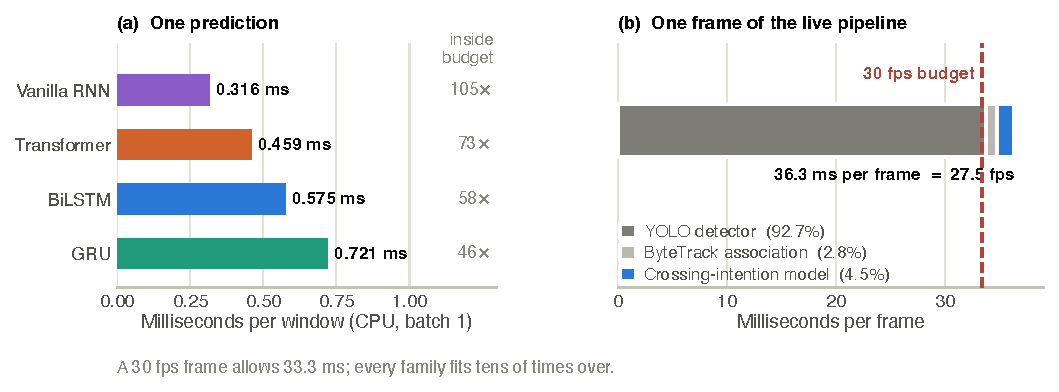
\includegraphics[width=\textwidth]{figures/fig8_latency.pdf}
\caption{Inference cost, measured on an Apple M4. (\textbf{a}) One crossing-intention prediction, per family, on CPU at batch 1, with the number of times each fits inside a 30\,fps frame budget. (\textbf{b}) Where a frame's time actually goes in the live pipeline: the detector dominates and the intention model is a rounding error, so the pipeline is detection-bound.\label{fig:latency}}
\end{figure}

\subsection{Detector-in-the-Loop Robustness}
\label{sec:detector}

Benchmark numbers on PIE are computed from annotated boxes. A deployed system receives boxes from a detector, so we measured what that substitution costs. On two test-set clips covering 98 pedestrians and 311 windows, replacing annotated boxes with detector boxes (mean IoU 0.75) moved AUC only from 0.962 to 0.953 per window and from 0.958 to 0.948 per pedestrian, with the decision flipping across the threshold in 10 of 311 windows (3\%). Prediction is robust to realistic box noise.

The weak links lie earlier in the pipeline. Detector recall is 88\% of pedestrians, so roughly one in eight is never covered well enough to be scored at all, a safety gap worth stating explicitly. Identity fragmentation is worse: a pedestrian's dominant ByteTrack identity covers a mean of only 39\% of its matched frames, and 59\% of windows carry a competing identity. A deployed system would need substantially stronger re-identification. These are detector and tracker engineering problems, separate from the crossing-intention model, but they are what would actually limit the system in the field.

One caveat bounds this experiment. Each detector window is assembled from the best-IoU detection per frame, matched against the annotated box. That isolates box-localization noise, which is what we set out to measure, but it also removes exactly the association errors quantified in the previous paragraph. The reported 0.009 AUC drop is therefore a lower bound on end-to-end degradation, not an estimate of it.

\subsection{Qualitative Behaviour}
\label{sec:qualitative}

Figure~\ref{fig:qualitative} shows the complete pipeline running on two test-set scenes. Boxes come from the detector and tracker rather than from annotations, and the probabilities are the same five-seed BiLSTM-F1 ensemble reported in Table~\ref{tab:families}, at its validation-tuned threshold of 0.516. Both pedestrians are annotated in PIE, so each verdict can be checked against ground truth rather than judged by eye.

Panel~(a) is the leakage-free protocol made visible. The model commits to ``will cross'' at $p = 0.71$ a second and a half before this pedestrian steps off the kerb, while they are still standing on it. Under the track-end protocol audited in Section~\ref{sec:leakage-results}, a window for the same pedestrian could have been drawn from frames in which they were already in the road; here that is impossible by construction, and what the picture shows is anticipation rather than recognition. Panel~(b) is the complementary case, and the harder one. To any rule based on position it is the same picture: a person standing at a kerb beside a marked crosswalk, which is where crossings begin. This one is a worker who does not cross, and the model correctly leaves him at $p = 0.31$. What separates the two panels is the motion history behind each box, not where either pedestrian is standing.

These two frames are illustrative, not representative, and we chose them deliberately from the pool of pedestrians whose ground truth we could verify. The corresponding error rates are the measured ones reported in Section~\ref{sec:detector}: detector recall of 88\%, a dominant-track purity of 39\%, and decisions that flip in 3\% of windows under detector box noise. Across the two clips shown here, the ensemble scores 134 true positives, 16 false positives, 19 false negatives, and 270 true negatives over 439 windows (accuracy 0.920, F1 0.884), close to and slightly above its performance on the full test set. Video~S1 shows the same pipeline running continuously over 26\,s of test clip video\_0012, which conveys something a still cannot: the probability for a given track is not static but firms up as the pedestrian's approach to the kerb resolves.

\begin{figure}[H]
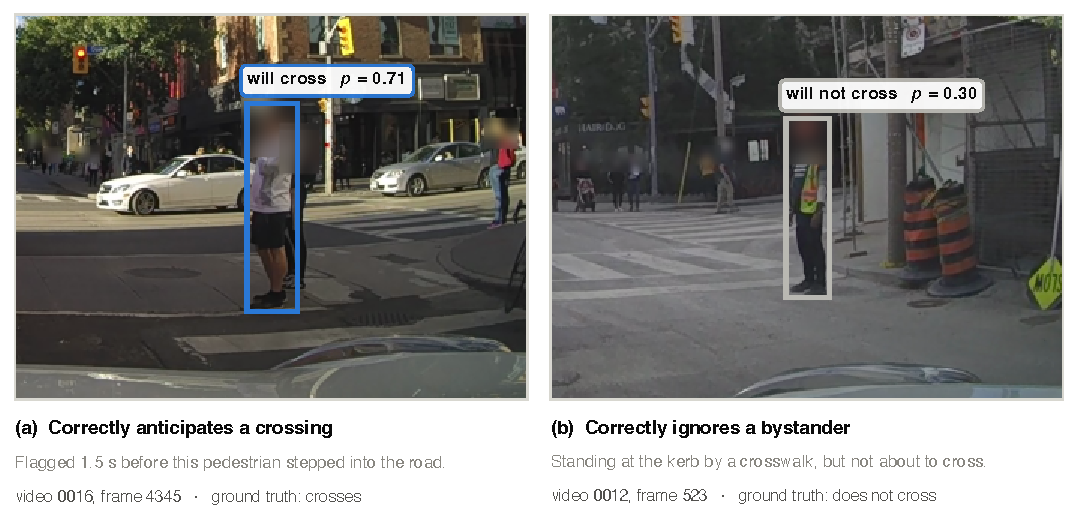
\includegraphics[width=\textwidth]{figures/fig9_qualitative.pdf}
\caption{The full detection-to-prediction pipeline on two PIE test-set scenes, with boxes from YOLO and ByteTrack rather than from annotations, and probabilities from the five-seed BiLSTM-F1 ensemble at threshold 0.516. (\textbf{a}) A pedestrian correctly flagged as about to cross, 1.5\,s before stepping into the road. (\textbf{b}) A worker standing at a kerb beside a crosswalk, correctly not flagged. The two scenes are near-identical in pedestrian position and opposite in outcome. Both verdicts agree with PIE's ground-truth crossing labels. Faces were blurred before publication; the blur is applied to the image data itself. Aggregate error rates for these clips are given in the text and in Section~\ref{sec:detector}.\label{fig:qualitative}}
\end{figure}

%=================================================================
\section{Discussion}
\label{sec:discussion}

\subsection{Two Streams Are Enough, and We Can Say Why}

Two cheap inputs reach F1 within about 0.02 of the multimodal ceiling and the highest AUC in the standard-protocol table, at a small fraction of the feature-extraction cost. We do not claim to be first to find this. PedCMT~\citep{chen2024pedcmt} and the pose-free ablation of GTransPDM~\citep{xie2025gtranspdm} reported comparable results from the same two streams, and~\citet{achaji2022attention} made the case from box geometry alone. What this paper adds is that the finding survives a leakage-free protocol and full statistical scrutiny and, more usefully, an account of \emph{why} it holds.

The explanation comes from putting two results side by side. Removing ego-speed collapses the model, while replacing its temporal encoder with three quite different alternatives changes nothing measurable. Together these say that the predictive content is concentrated in the ego-speed profile and coarse box dynamics, and that it is legible within half a second. There is no long-range structure for a heavier encoder to find. That is a claim about the task, not about our particular implementation, and it explains why so many differently architected models cluster within a few points of one another on this benchmark.

For a practitioner the implication is direct: the effort spent adding a pose estimator or an optical-flow network to a PIE-style crossing predictor is likely better spent elsewhere in the pipeline, and Section~\ref{sec:detector} suggests where.

\subsection{Model Choice Is a Metric-Priority Question}

The architecture comparison resolves differently depending on which metric leads. On AUC, a searched Transformer wins. On F1, all four families tie. Neither result is wrong; they are answers to different questions, and a paper that reported only one of them would be telling half the story.

This has a practical consequence. Given the F1-first hierarchy and near-identical latency, there is no performance argument for preferring a Transformer here, and there are reasons to prefer a small recurrent model, which is simpler to deploy, quicker to train, and in the case of the un-gated network, both the smallest and the fastest in the study. It also has a methodological consequence: an architecture comparison that reports a single metric, from a single seed, with unequal search budgets can produce a headline in either direction. Ours could have.

\subsection{The Cost of an Unaudited Protocol}

That two-thirds of crossing pedestrians were observed mid-crossing under a widely used windowing rule is, we think, the most transferable finding here. The dataset authors' own recent benchmark notes a related misalignment between how intention and action samples are anchored~\citep{rasouli2024diving}; our contribution is to quantify the consequence on PIE and to show what changes when it is removed.

The specific ways the artifact showed itself may help others recognize it. Convergence was implausibly fast (epoch 3 rather than 17). Static box geometry alone separated the classes at effect sizes above 0.6. And the model was insensitive to prediction horizon, which in hindsight is the clearest tell of all, since a model that genuinely respects a horizon must find a longer one harder. Any of these should prompt an audit. The audit itself is cheap: it needs only a per-frame event annotation that PIE already provides.

\subsection{What Would Actually Limit a Deployment}

The predictor is not the bottleneck. It runs in well under a millisecond, tolerates realistic detector box noise with a 0.009 AUC drop, and is a few percent of per-frame cost. Detection recall of 88\% and a dominant-track purity of 39\% are the numbers that would matter in a vehicle, and neither is a property of the model this paper is about. We think that reframing is useful: the marginal safety return on a better crossing-intention model appears smaller than the return on better perception, at least at this point on the curve.

\subsection{Limitations}
\label{sec:limitations}

The dominant feature is partly a measurement of the driver. Ego-speed encodes the ego-driver's own anticipation. An instrumented vehicle slows for a pedestrian the driver expects to cross. It is a legitimate signal at inference time, and it is available on any production vehicle, but it is not purely a measurement of the pedestrian, and a model leaning on it inherits some of the driver's judgment. The field has independently flagged this driver-side bias in yielding scenarios~\citep{azarmi2024featureimportance}. A speed-perturbation robustness study is the natural next step and we have not run it.

The equivalence we report is also horizon-bounded. Section~\ref{sec:horizon} shows the un-gated network beginning to fall behind at a two-second observation window. ``Gating is unnecessary'' is a statement about a 0.5\,s window, not about recurrent architectures in general.

The detector-in-the-loop study is indicative rather than conclusive. Two clips, 98 pedestrians, and an oracle-guided box association make the reported degradation a lower bound, not a deployment estimate.

Statistical power at the seed level is low. Five seeds cannot support a strong claim about seed-level variance, which is exactly why the paired and pedestrian-cluster bootstraps over the test windows, rather than seed-level tests, carry the argument.

Finally, every result here comes from a single dataset. Cross-dataset validation is under way but is not reported as a result of this paper, and the reason is instructive rather than incidental: JAAD does not record ego-vehicle speed at all, and the dataset authors note that its poor ego-motion severely degrades dynamics-dependent models~\citep{rasouli2024diving}. A JAAD replication can therefore validate the leakage audit and the architecture isolation, but structurally cannot test the ego-speed finding, which is our headline. A nuScenes-based~\citep{caesar2020nuscenes} evaluation with self-derived crossing labels can test the full two-stream model, at the cost of labels that are ours rather than the dataset's. We report this as ongoing work and claim no generalization beyond PIE here.

%=================================================================
\section{Conclusions}
\label{sec:conclusions}

We revisited pedestrian crossing-intention prediction on PIE and found that a widely used windowing protocol lets the crossing event into the observation window for 67.9\% of crossing pedestrians, turning much of the benchmark into detection rather than prediction. Re-anchoring the extraction at PIE's own crossing point removes the leakage entirely and, as a side effect, enlarges the dataset 3.5-fold.

On that leakage-free protocol, a model using only a pedestrian bounding box and the ego-vehicle's speed reaches F1 0.844--0.852 and the highest AUC among published results on the standard split, at sub-millisecond inference latency and with two input streams rather than the three to seven used by recent multimodal systems. Ego-speed is the dominant predictor: removing it costs 0.18 AUC. The temporal architecture, by contrast, is close to irrelevant. A bidirectional LSTM, a searched Transformer, a GRU, and an un-gated vanilla RNN, trained under one identical engine, are statistically indistinguishable on the primary metric, and even removing gating altogether costs nothing over a half-second window. The input signal, not the architecture, decides. No comparison here rests on a point estimate: each is backed by a paired bootstrap over pedestrian clusters, and the headline model is further checked by leave-one-set-out cross-validation, five-seed variance, a documented hyperparameter search, and a detector-in-the-loop test, under a metric hierarchy that places F1 first.

Three directions follow. The most pressing is cross-dataset validation, which is under way and is complicated by the fact that the obvious second dataset lacks the signal this paper identifies as decisive. The second is probing how far the ego-speed result depends on the ego-driver's own anticipation, which a speed-perturbation study would begin to answer. The third is the perception front end: on the evidence of Section~\ref{sec:detector}, detector recall and track identity, not the intention model, are what would limit such a system in a vehicle.
%=================================================================
\vspace{6pt}

\supplementary{The following supporting information can be downloaded at \linksupplementary{s1}: Video S1, the complete detection-to-prediction pipeline running on PIE test clip video\_0012 (26\,s, annotated with per-track crossing probabilities and ego-vehicle speed). Faces are blurred in the video as they are in Figure~\ref{fig:qualitative}.}

\authorcontributions{Conceptualization, methodology, software, validation, formal analysis, investigation, data curation, writing---original draft preparation, writing---review and editing, and visualization: [author initials]. Supervision: [supervisor initials]. All authors have read and agreed to the published version of the manuscript. (PLACEHOLDER: complete once authorship is finalized.)}

\funding{This research received no external funding.}

\institutionalreview{Not applicable. This study used the publicly available PIE dataset~\citep{rasouli2019pie} and did not involve new experiments on humans or animals. The video frames reproduced in Figure~\ref{fig:qualitative} are from that dataset; the face region of every person detected in those frames was irreversibly blurred before publication.}

\informedconsent{Not applicable.}

\dataavailability{The PIE dataset is publicly available~\citep{rasouli2019pie}. The leakage-free extraction protocol, training engine, and evaluation code developed for this study are available from the authors on reasonable request. (PLACEHOLDER: replace with the public repository URL upon release.)}

\conflictsofinterest{The authors declare no conflicts of interest.}

\abbreviations{Abbreviations}{%
The following abbreviations are used in this manuscript:\\

\noindent
\begin{tabular}{@{}ll}
ADAS & Advanced Driver-Assistance System\\
AUC & Area Under the (ROC) Curve\\
BiLSTM & Bidirectional Long Short-Term Memory\\
GRU & Gated Recurrent Unit\\
IoU & Intersection over Union\\
LOSO & Leave-One-Set-Out (cross-validation)\\
OBD & On-Board Diagnostics\\
PIE & Pedestrian Intention Estimation (dataset)\\
PR-AUC & Precision--Recall Area Under the Curve\\
RNN & Recurrent Neural Network\\
TTE & Time-To-Event
\end{tabular}
}

%=================================================================
\reftitle{References}

\bibliography{references}

\PublishersNote{}
\end{document}
